\documentclass[10pt]{article}
\usepackage[right=2cm,left=2cm,top=2cm,bottom=3cm]{geometry}
\usepackage[utf8]{inputenc}
\usepackage[spanish]{babel}
\usepackage{amsmath}
\usepackage{color}
\usepackage{listings}
\usepackage{graphicx}
%\usepackage{multicol}

%COLORES CODIGO
\definecolor{gray97}{gray}{.97}
\definecolor{gray75}{gray}{.75}
\definecolor{gray45}{gray}{.45}
\definecolor{claregreen}{RGB}{4,180,95}
\definecolor{darkblue}{rgb}{0.0,0.0,0.6}


\lstset{ frame=Ltb,
     framerule=0pt,
     aboveskip=0.5cm,
     framextopmargin=3pt,
     framexbottommargin=3pt,
     framexleftmargin=0.4cm,
     framesep=0pt,
     rulesep=.4pt,
     backgroundcolor=\color{gray97},
     rulesepcolor=\color{black},
     %
     stringstyle=\ttfamily,
     showstringspaces = false,
     basicstyle=\small\ttfamily,
     commentstyle=\color{gray45},
     keywordstyle=\bfseries,
     %
     numbers=left,
     numbersep=15pt,
     numberstyle=\tiny,
     numberfirstline = false,
     breaklines=true,
   }

% minimizar fragmentado de listados
\lstnewenvironment{listing}[1][]
   {\lstset{#1}\pagebreak[0]}{\pagebreak[0]}

%LENGUAJE OZ
\lstdefinelanguage{OZ}
{
  morestring=[b]',
  morecomment=[s]{\%}{\%},
  stringstyle=\color{claregreen},
  keywordstyle=\color{blue}\bfseries,
  morekeywords={proc, end, \$},% list your attributes here
  emph={REQUIRED},
  emphstyle=\color{red}
}

%MODO CONSOLA
\lstdefinestyle{consola}
   {basicstyle=\scriptsize\bf\ttfamily,
    backgroundcolor=\color{gray75},
   }




%opening
\title{Simulación de Eventos Discretos.\\ \emph{Informe de Modelo e Implementación.} \\ \textbf{Simulación de Fallas de Máquinas.} }
\author{\textbf{María Andrea Cruz Blandon  0831816.} \\ \textbf{Edgar Andres Moncada 0832294.  }\\ \textbf{Luis Felipe Vargas Rojas 0836342. }}
\date{\today}







\begin{document}
\maketitle

\section{Análisis del Sistema y del Problema.}
\subsection{Descripción del Sistema}
El sistema se compone de un conjunto de maquinas, las maquinas procesan la entrada y generan una salida, en el  sistema no existe conexión entre las maquinas cada una procesa su input independientemente de las otras, las maquinas se mantienen encendidas 8 horas del día, es decir que el rendimiento total semanal se calcula con la formula $8*5*50$ donde 8 son las  horas del dia , 5 son los dias de la  semana, y 50 es el número de maquinas.
\subsection{Descripción Gráfica del Sistema}
\begin{center}

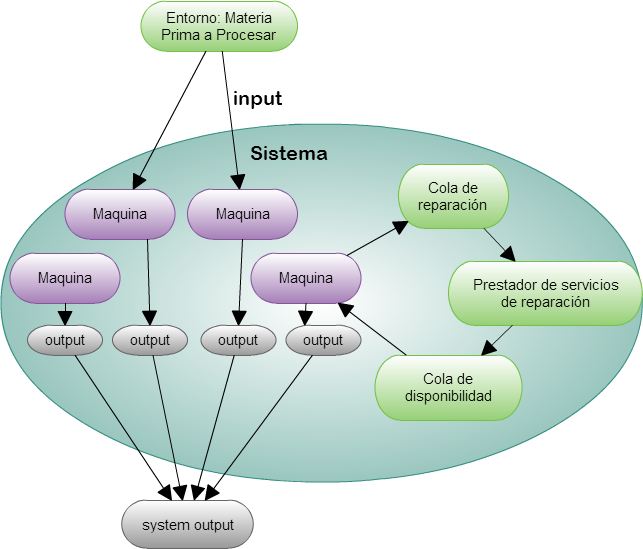
\includegraphics[scale=0.50]{Simulacion.png}

Figura1.\emph{Comportamiento del Sistema}
\end{center}
\section{Modelo de Simulación.}

\section{Diseño y Analisis de Escenarios.} 

\section{Implementación del Modelo.}

\section{Conclusiones.}



\end{document}
